\documentclass[12pt]{article}
\usepackage[utf8]{inputenc}
\usepackage{booktabs}
\usepackage{geometry}
\usepackage{graphicx}
\geometry{a4paper, margin=1in}
\title{Results of Fisher's Combined Test}
\author{Sara Fraija}
\date{\today}
\begin{document}
\maketitle
\section{Results}

\begin{table}[h!]
\centering
\resizebox{\textwidth}{!}{%
\begin{tabular}{l c c c c c c}
\toprule
\textbf{GRB} & \textbf{Transit} & \textbf{Significance} & \textbf{Corrected Significance} & \textbf{p-value} & \textbf{Corrected p-value} & \textbf{PDF} \\ \midrule
GRB170708046 & 1 & 0.98 & 0.11 & 1.635e-01 & 4.543e-01 & 2.468e-01 \\
GRB170816599 & 1 & 1.70 & 1.16 & 4.457e-02 & 1.238e-01 & 9.405e-02 \\
GRB170222209 & 1 & 0.68 & 0.00 & 2.483e-01 & 1.000e+00 & 3.166e-01 \\
GRB170403583 & 1 & 0.00 & 0.00 & 5.000e-01 & 1.000e+00 & 3.989e-01 \\
GRB170826369 & 1 & 1.64 & 0.22 & 5.050e-02 & 4.112e-01 & 1.040e-01 \\
GRB190515190 & 1 & 0.00 & 0.00 & 5.000e-01 & 1.000e+00 & 3.989e-01 \\
GRB150110923 & 1 & 1.61 & 1.61 & 5.370e-02 & 5.370e-02 & 1.092e-01 \\
GRB150922234 & 1 & 2.31 & 2.31 & 1.044e-02 & 1.044e-02 & 2.768e-02 \\
GRB160726065 & 1 & 0.65 & 0.65 & 2.578e-01 & 2.578e-01 & 3.230e-01 \\
GRB170325331 & 1 & 0.00 & 0.00 & 5.000e-01 & 5.000e-01 & 3.989e-01 \\
GRB180715755 & 1 & 0.58 & 0.58 & 2.810e-01 & 2.810e-01 & 3.372e-01 \\
GRB180718082 & 1 & 1.58 & 1.58 & 5.705e-02 & 5.705e-02 & 1.145e-01 \\
GRB181125371 & 1 & 0.00 & 0.00 & 5.000e-01 & 5.000e-01 & 3.989e-01 \\
GRB190427190 & 1 & 2.55 & 2.55 & 5.386e-03 & 5.386e-03 & 1.545e-02 \\
GRB201008443 & 1 & 2.22 & 2.22 & 1.321e-02 & 1.321e-02 & 3.394e-02 \\
GRB201221963 & 1 & 0.00 & 0.00 & 5.000e-01 & 5.000e-01 & 3.989e-01 \\
GRB210323918 & 1 & 0.66 & 0.66 & 2.546e-01 & 2.546e-01 & 3.209e-01 \\
GRB170817529 & 1 & 2.72 & 2.72 & 3.264e-03 & 3.264e-03 & 9.871e-03 \\
GRB141205337 & 1 & 1.05 & 1.05 & 1.469e-01 & 1.469e-01 & 2.299e-01 \\
GRB150101270 & 1 & 1.05 & 1.05 & 1.469e-01 & 1.469e-01 & 2.299e-01 \\
GRB150101641 & 1 & 1.44 & 1.44 & 7.493e-02 & 7.493e-02 & 1.415e-01 \\
GRB150120123 & 1 & 2.06 & 2.06 & 1.970e-02 & 1.970e-02 & 4.780e-02 \\
GRB151228129 & 1 & 0.27 & 0.27 & 3.936e-01 & 3.936e-01 & 3.847e-01 \\
GRB151229285 & 1 & 1.06 & 1.06 & 1.446e-01 & 1.446e-01 & 2.275e-01 \\
GRB160612842 & 1 & 0.38 & 0.38 & 3.520e-01 & 3.520e-01 & 3.712e-01 \\
GRB160624477 & 1 & 0.90 & 0.90 & 1.841e-01 & 1.841e-01 & 2.661e-01 \\
GRB160821937 & 1 & 1.93 & 1.93 & 2.680e-02 & 2.680e-02 & 6.195e-02 \\
GRB170318644 & 1 & 0.00 & 0.00 & 5.000e-01 & 5.000e-01 & 3.989e-01 \\
GRB170803729 & 1 & 0.52 & 0.52 & 3.015e-01 & 3.015e-01 & 3.485e-01 \\
GRB180204109 & 1 & 1.75 & 1.75 & 4.006e-02 & 4.006e-02 & 8.628e-02 \\
GRB180418281 & 1 & 1.10 & 1.10 & 1.357e-01 & 1.357e-01 & 2.179e-01 \\
GRB180805543 & 1 & 0.06 & 0.06 & 4.761e-01 & 4.761e-01 & 3.982e-01 \\
GRB201214672 & 1 & 2.87 & 2.87 & 2.052e-03 & 2.052e-03 & 6.491e-03 \\
GRB210827416 & 1 & 0.27 & 0.27 & 3.936e-01 & 3.936e-01 & 3.847e-01 \\
GRB211024065 & 1 & 0.00 & 0.00 & 5.000e-01 & 5.000e-01 & 3.989e-01 \\
GRB220412713 & 1 & 1.01 & 1.01 & 1.562e-01 & 1.562e-01 & 2.396e-01 \\
GRB220418720 & 1 & 0.83 & 0.83 & 2.033e-01 & 2.033e-01 & 2.827e-01 \\
GRB220511571 & 1 & 1.60 & 1.60 & 5.480e-02 & 5.480e-02 & 1.109e-01 \\
GRB220617772 & 1 & 0.27 & 0.27 & 3.936e-01 & 3.936e-01 & 3.847e-01 \\
GRB221120895 & 1 & 0.71 & 0.71 & 2.389e-01 & 2.389e-01 & 3.101e-01 \\
GRB230228244 & 1 & 0.00 & 0.00 & 5.000e-01 & 5.000e-01 & 3.989e-01 \\
GRB230512269 & 1 & 0.84 & 0.84 & 2.005e-01 & 2.005e-01 & 2.803e-01 \\
GRB230812790 & 1 & 0.37 & 0.37 & 3.557e-01 & 3.557e-01 & 3.725e-01 \\
GRB170708046 & 2 & 0.84 & -0.14 & 2.005e-01 & 5.568e-01 & 2.803e-01 \\
GRB170816599 & 2 & 1.95 & 1.47 & 2.559e-02 & 7.108e-02 & 5.959e-02 \\
GRB170206453 & 2 & 1.70 & 0.36 & 4.457e-02 & 3.578e-01 & 9.405e-02 \\
GRB170222209 & 2 & 2.05 & 1.06 & 2.018e-02 & 1.435e-01 & 4.879e-02 \\
GRB170403583 & 2 & 1.59 & 0.51 & 5.592e-02 & 3.044e-01 & 1.127e-01 \\
GRB170826369 & 2 & 3.04 & 2.34 & 1.183e-03 & 9.631e-03 & 3.928e-03 \\
GRB190515190 & 2 & 2.07 & 0.93 & 1.923e-02 & 1.757e-01 & 4.682e-02 \\
GRB200605762 & 2 & 0.99 & -0.37 & 1.611e-01 & 6.443e-01 & 2.444e-01 \\
GRB150922234 & 2 & 1.85 & 1.85 & 3.216e-02 & 3.216e-02 & 7.206e-02 \\
GRB160726065 & 2 & 0.60 & 0.60 & 2.743e-01 & 2.743e-01 & 3.332e-01 \\
GRB170325331 & 2 & 1.00 & 1.00 & 1.587e-01 & 1.587e-01 & 2.420e-01 \\
GRB180715755 & 2 & 0.27 & 0.27 & 3.936e-01 & 3.936e-01 & 3.847e-01 \\
GRB180718082 & 2 & 2.90 & 2.90 & 1.866e-03 & 1.866e-03 & 5.953e-03 \\
GRB181125371 & 2 & 0.98 & 0.98 & 1.635e-01 & 1.635e-01 & 2.468e-01 \\
GRB190427190 & 2 & 0.00 & 0.00 & 5.000e-01 & 5.000e-01 & 3.989e-01 \\
GRB201008443 & 2 & 2.21 & 2.21 & 1.355e-02 & 1.355e-02 & 3.470e-02 \\
GRB201221963 & 2 & 0.75 & 0.75 & 2.266e-01 & 2.266e-01 & 3.011e-01 \\
GRB210323918 & 2 & 0.78 & 0.78 & 2.177e-01 & 2.177e-01 & 2.943e-01 \\
GRB170817529 & 2 & 1.12 & 1.12 & 1.314e-01 & 1.314e-01 & 2.131e-01 \\
GRB141205337 & 2 & 2.19 & 2.19 & 1.426e-02 & 1.426e-02 & 3.626e-02 \\
GRB150101270 & 2 & 2.97 & 2.97 & 1.489e-03 & 1.489e-03 & 4.847e-03 \\
GRB150101641 & 2 & 0.74 & 0.74 & 2.296e-01 & 2.296e-01 & 3.034e-01 \\
GRB150110923 & 2 & 2.06 & 2.06 & 1.970e-02 & 1.970e-02 & 4.780e-02 \\
GRB151229285 & 2 & 1.02 & 1.02 & 1.539e-01 & 1.539e-01 & 2.371e-01 \\
GRB160624477 & 2 & 1.92 & 1.92 & 2.743e-02 & 2.743e-02 & 6.316e-02 \\
GRB160714097 & 2 & 1.22 & 1.22 & 1.112e-01 & 1.112e-01 & 1.895e-01 \\
GRB170318644 & 2 & 1.23 & 1.23 & 1.093e-01 & 1.093e-01 & 1.872e-01 \\
GRB170803729 & 2 & 0.92 & 0.92 & 1.788e-01 & 1.788e-01 & 2.613e-01 \\
GRB171007498 & 2 & 0.00 & 0.00 & 5.000e-01 & 5.000e-01 & 3.989e-01 \\
GRB180204109 & 2 & 0.93 & 0.93 & 1.762e-01 & 1.762e-01 & 2.589e-01 \\
GRB180402406 & 2 & 2.02 & 2.02 & 2.169e-02 & 2.169e-02 & 5.186e-02 \\
GRB180418281 & 2 & 2.18 & 2.18 & 1.463e-02 & 1.463e-02 & 3.706e-02 \\
GRB180805543 & 2 & 1.77 & 1.77 & 3.836e-02 & 3.836e-02 & 8.329e-02 \\
GRB191031891 & 2 & 0.52 & 0.52 & 3.015e-01 & 3.015e-01 & 3.485e-01 \\
GRB200415367 & 2 & 3.45 & 3.45 & 2.803e-04 & 2.803e-04 & 1.038e-03 \\
GRB200623138 & 2 & 0.00 & 0.00 & 5.000e-01 & 5.000e-01 & 3.989e-01 \\
GRB201214672 & 2 & 2.20 & 2.20 & 1.390e-02 & 1.390e-02 & 3.547e-02 \\
GRB210618072 & 2 & 1.22 & 1.22 & 1.112e-01 & 1.112e-01 & 1.895e-01 \\
GRB210827416 & 2 & 0.00 & 0.00 & 5.000e-01 & 5.000e-01 & 3.989e-01 \\
GRB211024065 & 2 & 1.25 & 1.25 & 1.056e-01 & 1.056e-01 & 1.826e-01 \\
GRB220412713 & 2 & 1.26 & 1.26 & 1.038e-01 & 1.038e-01 & 1.804e-01 \\
GRB220418720 & 2 & 2.48 & 2.48 & 6.569e-03 & 6.569e-03 & 1.842e-02 \\
GRB220511571 & 2 & 2.51 & 2.51 & 6.037e-03 & 6.037e-03 & 1.709e-02 \\
GRB220617772 & 2 & 1.95 & 1.95 & 2.559e-02 & 2.559e-02 & 5.959e-02 \\
GRB221120895 & 2 & 0.55 & 0.55 & 2.912e-01 & 2.912e-01 & 3.429e-01 \\
GRB230228244 & 2 & 1.22 & 1.22 & 1.112e-01 & 1.112e-01 & 1.895e-01 \\
GRB230512269 & 2 & 0.00 & 0.00 & 5.000e-01 & 5.000e-01 & 3.989e-01 \\
GRB230812790 & 2 & 1.30 & 1.30 & 9.680e-02 & 9.680e-02 & 1.714e-01 \\
\bottomrule
\end{tabular}%
}
\caption{Lista de GRBs con sus Tránsitos, Significancias, Significancias Corregidas, p-values, p-values Corregidos y valores PDF.}
\end{table}


\begin{figure}[h!]
\centering
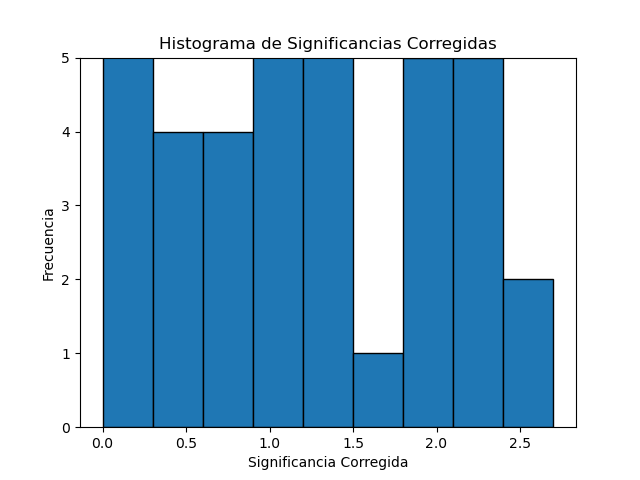
\includegraphics[width=0.45\textwidth]{2nd_TransitPSF_0.3corrected_significance_hist.png}
\hfill
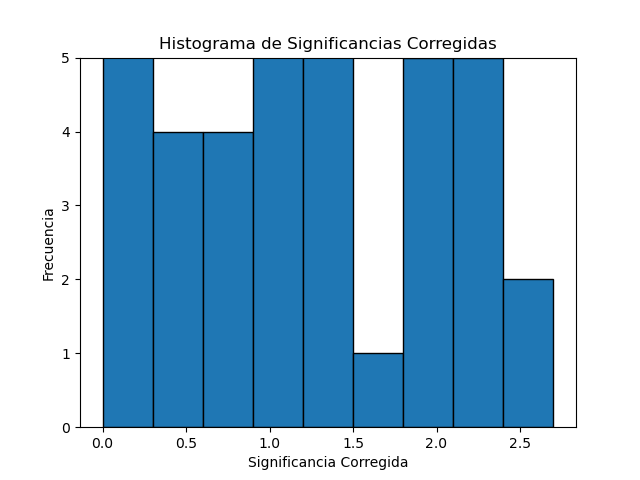
\includegraphics[width=0.45\textwidth]{2nd_TransitPSF_0.3corrected_significance_hist.png}
\caption{Histograma de Significancias (izquierda) y de Significancias Corregidas (derecha).}
\end{figure}


\section*{Conclusion}
Fisher's combined test integrates individual p-values to evaluate a global hypothesis. 
In this analysis, the test statistic obtained was $X^2 = 416.378$ with 182 degrees of freedom. 
For a significance level of 0.05, the critical chi-square value is 214.477. 
Since $X^2$ is greater than the critical value, 
we reject the null hypothesis that the events are independent.
\newline
Additionally, the chi-square value was converted using a normal approximation:
\newline
Normal p-value: 3.554e-20 and Normal significance: 9.13 sigma.


\end{document}
